% Fig 3.22 Angular distribution of positrons from mu+ decay, W(theta) ∝ 1 + cos(theta):
% cardioid envelope with rays from the cusp (arrow length = decay probability),
% bold arrow = initial muon spin direction.
\documentclass[tikz,border=5pt]{standalone}
\usetikzlibrary{arrows.meta}
\usepackage{amsmath}
\usepackage{bm}
\usepackage{fontspec}
\setmainfont{Times New Roman}
\begin{document}
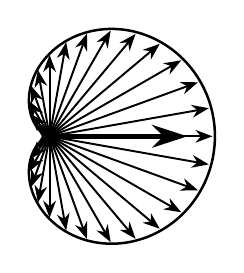
\begin{tikzpicture}[line width=0.7pt,>=Stealth]
\def\cx{0.6}\def\cy{1.4}\def\R{1.05}
% rays from the cusp to the envelope (length encodes the distribution)
\foreach \t in {0,10,...,150,210,220,...,350}{
  \draw[->] (\cx,\cy) --
    ({\cx+0.985*\R*(1+cos(\t))*cos(\t)},{\cy+0.985*\R*(1+cos(\t))*sin(\t)});
}
% cardioid envelope
\draw[line width=0.9pt] plot[domain=0:360,samples=240,smooth]
  ({\cx+\R*(1+cos(\x))*cos(\x)},{\cy+\R*(1+cos(\x))*sin(\x)});
% initial spin direction
\draw[line width=1.6pt,-{Stealth[length=4.5mm,width=2.9mm]}] (\cx,\cy) -- (2.35,1.4);
\end{tikzpicture}
\end{document}
